\FloatBarrier
Elektronen und Positronen haben durch ihre geringe Masse eine Sonderstellung
($m_{e^{\pm}} \approx 511$~keV/c$^2$, $m_{\mu} \approx 106$~MeV/c$^2$). Zusätzlich zum Energieverlust durch Ionisation und
Anregung hat daher der Energieverlust durch Bremsstrahlung eine größere Bedeutung:

\[-\left(\frac{\mathrm{d}E}{\mathrm{d}x}\right)_{\text{tot}} = -\left(\frac{\mathrm{d}E}{\mathrm{d}x}\right)_{\text{coll}}
-\left(\frac{\mathrm{d}E}{\mathrm{d}x}\right)_{\text{rad}} \]

Beim Energieverlust durch Ionisation und Anregung muss die Bethe-Bloch-Formel wegen der geringen
Masse modifiziert werden, aber auch, da eine Kollision zwischen quantenmechanisch nicht
unterscheidbaren Teilchen stattfindet. Die Ionisationsverluste steigen logarithmisch mit $E$ und
linear mit $Z$, die Bremsstrahlungsverluste dagegen in etwa linear mit $E$ und quadratisch mit $Z$.
Für hohe Energien (> 1~GeV) ist die Bremsstrahlung der dominierende Prozess.

\begin{figure}
	\centering
	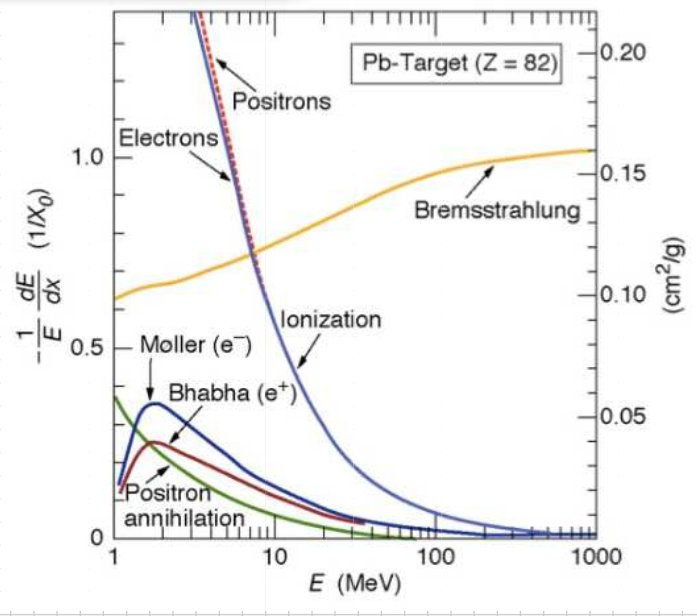
\includegraphics[width=0.5\textwidth]{energieverlust.jpg}
\end{figure}

% Elektronen/Positronen Streuung an Targetelektronen fällt unter Ionisation, wenn der Energieübertrag
% pro Kollision unter 0,255~MeV liegt und unter M\o ller-Streuung (Bhabha-Streuung), wenn er darüber
% liegt.

\FloatBarrier